% Full instructions available at:
% https://github.com/elauksap/focus-beamertheme

\documentclass{beamer}
\usetheme[numbering=none]{focus}
\usepackage[utf8x]{inputenc} %So spanish accents will work%
\usepackage{hyperref}
\usepackage{listings}
\usepackage{color}
\usepackage{verbatim}
\usepackage{inconsolata}

\definecolor{codegray}{rgb}{0.5,0.5,0.5}
\definecolor{codecyan}{RGB}{0, 255, 255}
\definecolor{codeyellow}{RGB}{240,219,78}

\lstdefinestyle{mystyle}{
    commentstyle=\color{codeyellow},
    keywordstyle=\color{magenta},
    numberstyle=\color{codegray},
    stringstyle=\color{codecyan},
    basicstyle=\ttfamily\small,
    breakatwhitespace=false,         
    breaklines=true,                 
    captionpos=b,                    
    keepspaces=true,
    showspaces=false,                
    showstringspaces=false,
    showtabs=false,                  
    tabsize=2
}

\lstdefinelanguage{JavaScript}{
keywords={typeof, new, true, false, catch, function, return, null, catch, switch, var, let, if, in, while, do, else, case, break, default, for, of},
ndkeywords={class, export, boolean, throw, implements, import, this},
ndkeywordstyle=\color{darkgray}\bfseries,
sensitive=false,
comment=[l]{//},
morecomment=[s]{/*}{*/},
morestring=[b]',
morestring=[b]",
morestring=[b]`,
}
\lstset{style=mystyle, escapeinside=||}
\title{Javascript}
\subtitle{Hour of Code 2018}

\titlegraphic{
\includegraphics[scale=0.13]{images/js_logo.png}}
\institute{Universidad de Valladolid}
\date{27 Oct 2018}

\begin{document}
\begin{frame}
        \maketitle
\end{frame}
    % PARAGRAPH SPACING. -----------------------------------------------------------------
    \setlength{\parskip}{\baselineskip}%
    \setlength{\parindent}{0pt}%

\begin{frame}{Qué es Javascript}
    	\pause
        Javascript (también llamado JS) es un lenguaje de programación originado en 1995.\pause

    	Es conocido principalmente por su uso en desarrollo web, permitiendo que un usuario pueda interaccionar con una pagina web.
\end{frame}
\begin{frame}{Qué es Javascript}
        Javascript es un lenguaje... \bigskip
        \begin{itemize}
            \item interpretado\pause
            \item que usa tipado débil\pause
            \item dinámico
    \end{itemize}
\end{frame}
    
\begin{frame}{Javascript es interpretado}
        \pause
        Un lenguaje \textbf{interpretado} es aquel que es traducido a código máquina a medida que se ejecuta, mientras que un lenguaje \textbf{compilado} es aquel que se traduce a código máquina antes de ejecutarse.\pause
        \centering
        
        Javascript es un lenguaje interpretado.
\end{frame}
    
\begin{frame}{Javascript usa tipado débil}
        \pause
        Un lenguaje que usa \textbf{tipado débil} no necesita declarar el tipo de sus variables explícitamente, mientras que un lenguaje que usa \textbf{tipado fuerte} necesita declarar el tipo que va a almacenar una variable de antemano.\pause
        \centering
        
        Javascript utiliza tipado débil.
\end{frame}
    
    
    
\begin{frame}{Javascript es dinámico}
        \pause
        Un lenguaje \textbf{dinámico} comprueba los tipos durante la ejecución del programa, mientras que un lenguaje \textbf{estático} los comprueba antes de la ejecución.\pause
        \centering
        
        Javascript es un lenguaje dinámico.
\end{frame}
\begin{frame}[fragile]{C: Compilado, tipado fuerte y estático}\pause
        \lstinputlisting[language=C++]{code_snippets/example.c}\centering
        
        Este programa ha de ser compilado con un compilador.
\end{frame}

\begin{frame}[fragile]{El mismo ejemplo, con Javascript}\pause
        \lstinputlisting[language=JavaScript]{code_snippets/example.js}\centering
\end{frame}

\begin{frame}{Cómo ejecutar Javascript}\pause
    Hay varias maneras de ejecutar Javascript. La mas accesible es desde vuestro navegador de preferencia (Firefox, Chrome...)\pause
    
    Abrid las herramientas de desarrollador (F12), y buscad la opción de consola.
    \begin{figure}
        \centering
        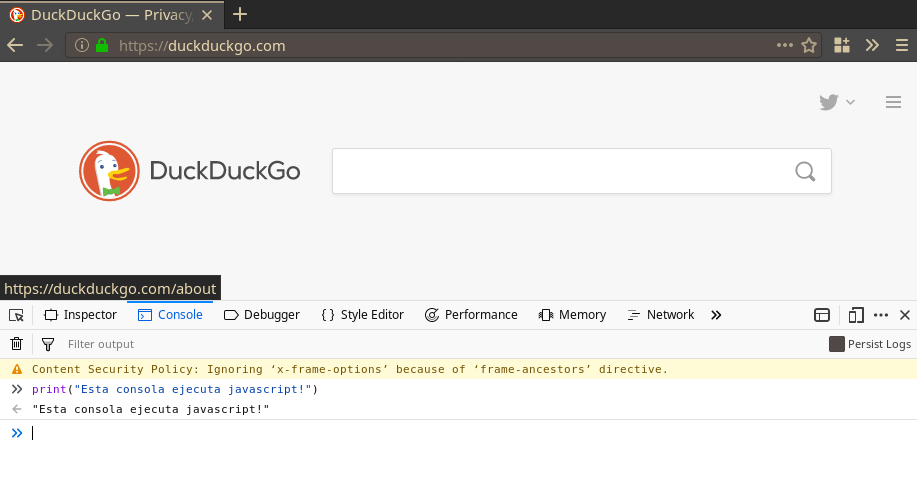
\includegraphics[width=0.75\textwidth]{images/firefox_dev.png}
    \end{figure}
\end{frame}

\begin{frame}{Como ejecutar Javascript}
Para este taller, vamos a utilizar JS Bin, un editor online de Javascript.
    
\centering\url{https://jsbin.com/?js,console}
\end{frame}

\begin{frame}{ECMAScript}
Antes de empezar con Javascript, deberíais saber esto...

ECMAScript es un estándar de lenguajes de programación, y Javascript es una implementación de dicho estándar.

ECMAScript se va actualizando con el tiempo con nuevas funcionalidades, y versiones antiguas de algunos navegadores pueden no estar actualizadas para soportar nuevas versiones de ECMAScript.
\end{frame}

\begin{frame}{ECMAScript}
En este taller, todo lo que os enseñe esta basado en ECMAScript 6 (También llamado ECMAScript 2015, o ES6) y esta soportado por todos los navegadores actuales.

En caso de que tengáis que soportar navegadores antiguos (Internet Explorer 11 y menor, por ejemplo), algunas partes de este taller no funcionarán.
\end{frame}

\begin{frame}[fragile]{Variables y constantes}
Hay varias maneras de crear variables en JavaScript:
\begin{itemize}
    \item {\verb|var|} para declarar una variable 
    \item {\verb|let|} para declarar una variable
    \item {\verb|const|} para declarar una constante
\end{itemize}

\end{frame}

\begin{frame}[fragile]{Var y let}
La diferencia entre {\verb|var|} y {\verb|let|} es simple.
\begin{itemize}
    \item {\verb|var|} define las variables a un nivel funcional (pertenecen a la función en la que se definen o, en caso de que no pertenezcan a ninguna, son globales)
    
    \item {\verb|let|} define las funciones a un nivel de bloque (pertenecen al bloque en el que se definen o, en caso de que no pertenezcan a ninguno, son globales)
\end{itemize}

Mostraremos ejemplos de esto mas adelante, cuando entendáis la sintaxis de JavaScript. En caso de duda, utilizad {\verb|let|} para evitar posibles problemas.
\end{frame}

\begin{frame}[fragile]{Const}
{\verb|const|} se utiliza para definir constantes. Esto implica que en la mayoría de los casos, una variable constante:
\begin{itemize}
    \item no puede ser reasignada
    \item no puede ser modificado*
\end{itemize}

Intentar hacer cualquiera de estas cosas a una constante va a resultar en un error.
\end{frame}

\begin{frame}{Tipos de datos}
En Javascript, tenemos los siguientes tipos de datos:\bigskip

\begin{columns}[t, onlytextwidth]
            \column{0.5\textwidth}
                \textbf{Primitivos:}
                \begin{itemize}
                    \item Number
                    \item String
                    \item Boolean
                    \item Null
                    \item Undefined
                    \item Symbol
                \end{itemize}
            
            \column{0.5\textwidth}
                \textbf{No primitivos:}
                \begin{itemize}
                    \item Object
                \end{itemize}
        \end{columns}
\end{frame}

\begin{frame}{Numbers}
Un \textbf{number} (Numero) es un tipo de dato numérico.

A diferencia de otros lenguajes, no hay distintos tipos dependiendo de si el numero es decimal o no, o de cuanto espacio se quiera reservar (short, int, long, double, float...)

En Javascript, solo hay un único tipo, number. Este es similar a un double en otros lenguajes de programación (64 bits, punto flotante)
\end{frame}

\begin{frame}[fragile]{Numbers}
\begin{lstlisting}[language=JavaScript]
let meaningOfLife = 42;
typeof(meaningOfLife); // "number"|\pause|

let floatingPoint = 3.141592;
typeof(floatingPoint); // "number"|\pause|

// Tambien puedes utilizar notacion cientifica
let exponentialNotation = 123e5; // 123 * (10^5) = 12300000|\pause|

// O hexadecimal (0x) y octal (0)
let hexadecimalNum = 0xFF; // 255
let octalNum = 0147 // 103
\end{lstlisting}    
\end{frame}

\begin{frame}[fragile]{Numbers: Casos especiales}
\begin{lstlisting}[language=JavaScript]
// Y que pasa si hago esto?
let divisionByZero = 1/0;|\pause| // Infinity|\pause|
let negativeDivisionByZero = -1/0; // -Infinity|\pause|

// Y un numero extremadamente grande?|\pause|
let giganticNumber = 1e9999; // Infinity
let giganticNegativeNumber = -1e9999; // -Infinity

// Infinity e -Infinity son de tipo number!
typeof(Infinity); // "number"
typeof(-Infinity); // "number"

// Y esto de aqui?
let divisionByTomato = 4 / "tomato";|\pause| // "NaN"
\end{lstlisting}    
\end{frame}

\begin{frame}{Numbers: Casos especiales}
NaN es un número especial. Como habréis notado, Javascript no suele devolver errores ante casos extraños.

Ya entraremos en detalle acerca de como Javascript maneja estos casos, pero por ahora centrémonos en NaN.\pause

NaN (Not a Number; No es un número) es un valor numérico que Javascript devuelve siempre que no encuentre un valor legal en una operación aritmética (como una string, con excepciones que ya mencionaremos)
\end{frame}

\begin{frame}[fragile]{Numbers: Operaciones}
\begin{lstlisting}[language=JavaScript]
let num1 = 9, num2 = 3;

// Operador de suma: +
let sumNums = num1 + num2; // 12

// Operador de resta: -
let substractNums = num1 - num2; // 6

// Operador de producto: *
let multiplyNums = num1 * num2; // 27

// Operador de division: /
let divideNums = num1 / num2; // 3

// Operador de resto: %
let reminderOfNums = num1 % num2; // 0
\end{lstlisting}
\end{frame}

\begin{frame}[fragile]{Numbers: Operaciones}
\begin{lstlisting}[language=JavaScript]
// Operador de incremento: ++
num1++; // num1 = 10;

// Operador de decremento: --
num2--; // num2 = 2;
\end{lstlisting}

\begin{block}{Cuidado! Operaciones con NaN}
Cualquier operación que tenga NaN en alguno de sus operandos devolverá NaN. 
\begin{lstlisting}
let someOperation = 46 + (38 % NaN) * 27; // NaN
\end{lstlisting}
\end{block}
\end{frame}

\begin{frame}[fragile]{Numbers: Punto flotante}
Recordad que en Javascript, \textbf{todos} los números son de punto flotante. Esto puede dar lugar a imprecisiones, y debéis de tener cuidado con estas.

\begin{lstlisting}[language=JavaScript]
0.1 + 0.2; // 0.30000000000000004

0.1 + 0.2 == 0.3; // false
\end{lstlisting}
\end{frame}

\begin{frame}[fragile]{Strings}
Un \textbf{String} es una cadena de caracteres usada para representar texto.

Puedes usar single quotes ('), double quotes (") o backticks (`) para delimitar un string, aunque estos últimos son un caso especial que ya mencionaremos.

\begin{lstlisting}[language=JavaScript]
let singleQuotes = 'Soy una cadena de caracteres!';
let doubleQuotes = "Yo tambien!";
let backTicks = `Y yo!`;

typeof(singleQuotes); // "string"
\end{lstlisting}
\end{frame}

\begin{frame}[fragile]{Strings}
En caso de que queráis utilizar alguno de los caracteres delimitantes en una string, tenéis dos formas de hacerlo:
\begin{itemize}
\item Utilizar un delimitador distinto: 
\begin{lstlisting}[language=JavaScript]
let doubleQuoteDelimited = "Uso ' y `!"

let singleQuoteDelimited = 'Y yo uso " y `!'

let backtickDelimited = `Tengo " y ' sin problemas!`
\end{lstlisting}
\item Escapar el caracter con \textbackslash:
\begin{lstlisting}[language=JavaScript]
let stringWithEscapedChar = "Esto \" funciona!"
\end{lstlisting}
\end{itemize}
\end{frame}

\begin{frame}[fragile]{Strings: Concatenación}
Las strings solo tienen un operador: concatenación (+)
\begin{lstlisting}[language=JavaScript]
let firstName = "Alberto";
let lastName = "Gonzalez";

let fullName = firstName + " " + lastName;
// fullName = "Alberto Gonzalez"
\end{lstlisting}
\begin{block}{Cuidado! No confundáis los operadores}
Tanto el operador de concatenación como el de adición utilizan el mismo símbolo (+), pero son dos operadores completamente distintos. Ya entraremos en detalle acerca de esto mas adelante.
\end{block}
\end{frame}

\begin{frame}[fragile]{Strings: template strings}
En caso de que quieras tener un string con valores de variables, usar template strings puede ser muy útil para facilitar la tarea.

Esto solo funciona si el string usa backticks como delimitador (`)\bigskip

\begin{lstlisting}[language=JavaScript]
let firstName = "Alberto";
let lastName = "Gonzalez";

let fullName = `${firstName} ${lastName}`;
// fullName = "Alberto Gonzalez"
\end{lstlisting}
\end{frame}

\begin{frame}[fragile]{Boolean}
Un \textbf{Boolean} (Booleano) es un tipo de dato que sólo tiene dos valores: true (verdadero) o false (falso).

\begin{lstlisting}[language=JavaScript]
let webDevRocks = true;
let javascriptIsGarbage = false;

typeof(webDevRocks); // "boolean"
typeof(javascriptIsGarbage); // "boolean"

\end{lstlisting}
\end{frame}

\begin{frame}{Boolean: Operadores booleanos}
Hay varios operadores booleanos: los operadores de comparación. Estos operadores comparan dos argumentos y siempre devuelven un booleano. \bigskip

\begin{columns}[t, onlytextwidth]
            \column{0.5\textwidth}
                \textbf{Comparadores normales}
                \begin{itemize}
                    \item Igualdad (==)
                    \item No igualdad (!=)
                    \item Mayor que (>)
                    \item Menor que (<)
                    \item Mayor o igual que (>=)
                    \item Menor o igual que (<=)
                \end{itemize}
            
            \column{0.5\textwidth}
                \textbf{Comparadores estrictos}
                \begin{itemize}
                    \item Igualdad (===)
                    \item No igualdad (!==)
                \end{itemize}
        \end{columns}
\end{frame}

\begin{frame}[fragile]{Boolean: Operadores booleanos}
\begin{lstlisting}[language=JavaScript]
4 == 7; // false
2 != 5; // true

3 > 4; // false
3 < 4; // true

2 > 2; // false
2 >= 2; // true
\end{lstlisting}
\end{frame}

\begin{frame}[fragile]{Boolean: Operadores booleanos}
Javascript hace varias conversiones de tipos por detrás cuando trabajas con tipos distintos.
\begin{lstlisting}[language=JavaScript]
3 > "5" // 3 > 5, false
4 == "4" // 4 == 4, true
\end{lstlisting}

Para evitar conversiones implícitas, utiliza los comparadores estrictos.
\begin{lstlisting}[language=JavaScript]
4 == "4" // 4 == 4, true
4 === "4" // false

2 != "2" // 2 != 2, false
2 !== "2" // true
\end{lstlisting}
Siempre que puedas, utiliza el comparador estricto para evitar problemas.


\end{frame}

\begin{frame}[fragile]{Null}
\textbf{null} es un tipo de dato que sólo tiene un valor: null.

null se usa para indicar que algo no tiene ningún valor; que esta vacío.

\begin{lstlisting}[language=JavaScript]
let void = null;

typeof(void); // "object" (por motivos de legacy)

\end{lstlisting}
\end{frame}

\begin{frame}[fragile]{Undefined}
\textbf{undefined} es un tipo de dato que solo tiene un valor: undefined.

Undefined se usa para indicar que algo no tiene ningún valor asignado.

\begin{lstlisting}[language=JavaScript]
let something;

typeof(something); // "undefined"
\end{lstlisting}
\end{frame}

\begin{frame}{Diferencia entre null y undefined}
null y undefined son dos cosas distintas, pese a parecer idénticas. Aquí tenéis un ejemplo visual.

    \begin{figure}
        \centering
        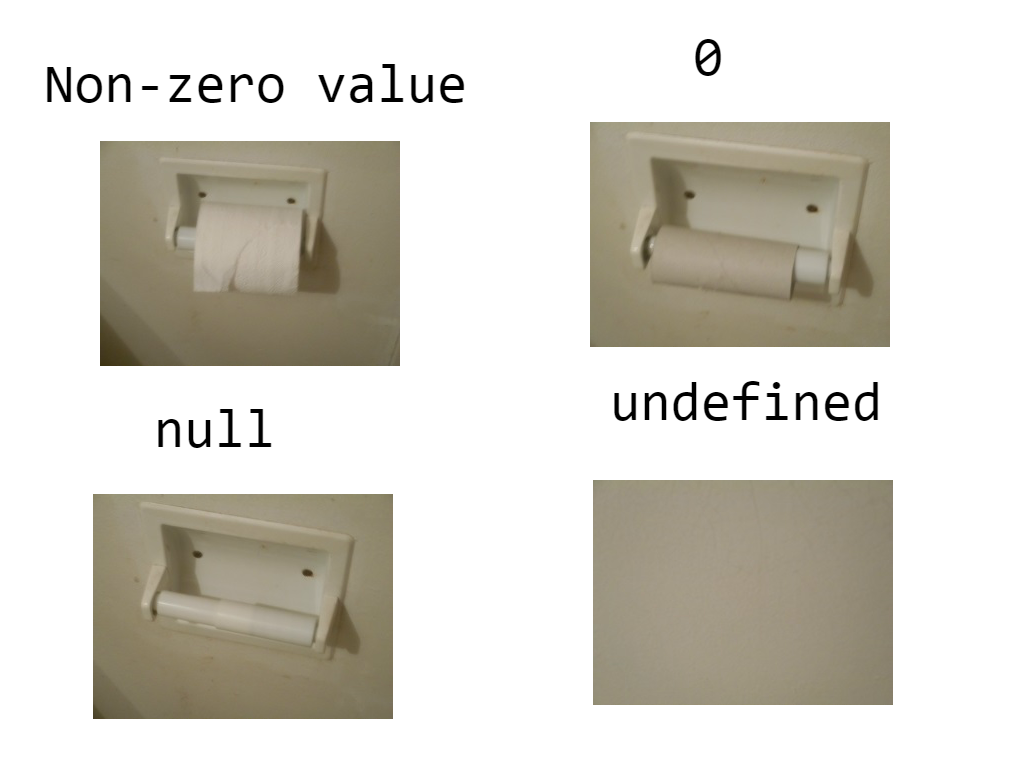
\includegraphics[width=0.7\textwidth]{images/undefinednull.png}
    \end{figure}
\end{frame}

\begin{frame}{Diferencia entre null y undefined}
\begin{itemize}
    \item Undefined indica que algo simplemente no esta ahí, y es el valor que toma cualquier variable por defecto.
    \item Null indica que el valor de algo es nulo, y has de asignarlo explícitamente a algo.
\end{itemize}
\end{frame}

\begin{frame}[fragile]{Conversiones implícitas}
Javascript hace conversiones entre tipos por detrás cuando trabajas con tipos distintos.

\begin{lstlisting}[language=JavaScript]
1 + "10" // "110"
1 + 10 // 11
"1" - 10 // "-9"
3 - "Tomato"  // NaN
"b"+"a"+(+"a")+"a" // "baNaNa"
1 / 0 + " and beyond!" // "Infinity and beyond!"
\end{lstlisting}
\end{frame}

\begin{frame}{Conversiones implícitas}
    \begin{figure}
        \centering
        
\includegraphics[width=\textwidth]{images/excuse_me.jpg}
    \end{figure}
\end{frame}

\begin{frame}{Conversiones implícitas}
Si estás sumando algo:
\begin{itemize}
    \item Si alguno de los operandos es una string, el otro se convierte en string y se concatenan
\end{itemize}

Si estas restando, multiplicando o dividiendo algo:
\begin{itemize}
    \item Si alguno de los operandos es una string, el otro se intenta convertir a número (En caso de que no se pueda, se convierte en NaN)
\end{itemize}
\end{frame}

\begin{frame}{Tipos de datos no primitivos}
Sólo hay un tipo de dato no primitivo: El tipo Object (objeto)

Un object es una colección de propiedades. Se definen utilizando llaves: \{ y \}

Cada propiedad tiene una "llave" (identificador) asignada, siguiendo el formato \textbf{\textit{llave : propiedad}}, y se separan con comas unos pares llave : propiedad de otros.
\end{frame}

\begin{frame}[fragile]{Objects}
\begin{lstlisting}[language=JavaScript]
market_stock = {"apples" : 4, "color" : "red"}

market_stock.apples // 4
market_stock.color // "red"
market_stock.precio // undefined

market_stock.apples-- // market_stock.apples = 3
market_stock.price = 4.95

market_stock // {apples: 3, color: "red", price: 4.95}
\end{lstlisting}
\end{frame}

\begin{frame}[fragile]{Arrays}

Un \textbf{array} es un tipo de objeto que te permite guardar múltiples valores distintos en una sola variable.

Una array se define con un par de corchetes [], separando los elementos con comas.

\begin{lstlisting}[language=JavaScript]
let someArray = [1, "manzana", 9, true];
typeof(someArray); // "object"
\end{lstlisting}


\end{frame}

\begin{frame}[fragile]{Arrays}
Puedes acceder a un elemento específico de un array especificando su índice (numeración basada en 0)

\begin{lstlisting}[language=JavaScript]
let someArray = [1, "manzana", 9, true];

someArray[0]; // 1
someArray[1]; // "manzana"
someArray[3]; // true
\end{lstlisting} 
\end{frame}


\begin{frame}{Estructuras de control}
Javascript tiene las siguientes estructuras de control.
\begin{itemize}
    \item if / else if / else
    \item while / do while
    \item for
    \item switch
    \item for each
    \item with
\end{itemize}
\end{frame}

\begin{frame}{If / Else if / Else}
La sentencia \textbf{if} te permite ejecutar una parte del código sólo si una condición se cumple de antemano. 

Una condición es cualquier sentencia que devuelva un valor booleano, o pueda convertirse en uno.

Si no se cumple dicha condición, puedes comprobar por condiciones adicionales usando \textbf{else if}, o puedes ejecutar código si no se cumple ninguna condición usando \textbf{else}.
\end{frame}

\begin{frame}[fragile]{If / Else if / Else}
\begin{lstlisting}[language=JavaScript]
let someNumber = 5;

if (someNumber < 3) {
    console.log("el numero es menor que 3.");
} else if (someNumber < 10) {
    console.log("el numero esta entre 3 y 9.");
} else {
    console.log("el numero es mayor a 9.");
}
\end{lstlisting}
\end{frame}

\begin{frame}{While / Do while}
La sentencia \textbf{while} te permite repetir la ejecución de una parte del código mientras se cumpla una condición.

La sintaxis de un bucle while es la siguiente:

\textbf{while (condicion) \{ código \} }

Una sentencia \textbf{do... while} es idéntica a un while, pero esta garantiza que el código se ejecutara al menos una vez, incluso si la condición no se cumple la primera vez.

\textbf{do \{ código \} while (condicion) }

\end{frame}

\begin{frame}[fragile]{While / Do while}
\begin{lstlisting}[language=JavaScript]
let counter = 5;

while(counter < 13){
    console.log(counter++);
}

do {
    console.log("Condicion imposible!");
} while (counter < 0)   
\end{lstlisting}
\end{frame}

\begin{frame}{For}
La sentencia \textbf{for} te permite repetir la ejecución de una parte del código un numero determinado de veces.

La sintaxis de un bucle for es la siguiente:

\textbf{for (contador; condición; paso) \{ código \} }

El contador es cualquier variable que se use para llevar la cuenta del numero de iteraciones del bucle.

La condición es que se ha de cumplir para que el bucle siga repitiéndose: Cuando la condición deja de cumplirse, el bucle para.

El paso indica de que manera quieres modificar el contador tras cada iteración del bucle.
\end{frame}

\begin{frame}[fragile]{For}
\begin{lstlisting}[language=JavaScript]
for(counter = 10; counter > 0; counter--){
    console.log("Lanzamiento en " + counter);
}
console.log("Despegue!");
\end{lstlisting}
\end{frame}

\begin{frame}[fragile]{Switch}
La sentencia \textbf{switch} te permite evaluar una expresión, y ejecutar un determinado código en base a dicha expresión.

La sintaxis de una sentencia switch es la siguiente:

\begin{lstlisting}[language=JavaScript]
switch (expresion) {
    case (condicion): 
        code
        break;
    case (condicion):
        code
        break;
    default:
        code
}\end{lstlisting}
\end{frame}

\begin{frame}[fragile]{Switch}
\begin{lstlisting}[language=JavaScript]
let fruit = "apple"
switch (fruit) {
    case banana: 
        console.log("Me quedan 3 platanos.")
        break;
    case apple:
        console.log("Me quedan 9 manzanas.")
        break;
    default:
        console.log("No me queda ninguna " + fruta)
}\end{lstlisting}
\end{frame}

\begin{frame}[fragile]{for each}
En JavaScript existen diferentes tipos de bucles \textbf{for each}, cada uno de los cuales tiene un comportamiento diferente:
\begin{itemize}
     \item for...of
    \item for...in
   
\end{itemize}
\end{frame}

\begin{frame}[fragile]{for...of}
La sentencia \textbf{for...of} crea un bucle que itera a través de los elementos de objetos iterables (incluyendo Array), ejecutando las sentencias de cada iteración con el valor del elemento que corresponda.\newline

La sintaxis de un bucle \textbf{for...of} es la siguiente:
\begin{lstlisting}[language=JavaScript]
for (variable of iterable) {
  code
}
\end{lstlisting}
\end{frame}

\begin{frame}[fragile]{for...of}
\begin{lstlisting}[language=JavaScript]
let iterable = [10, 20, 30]; //Array de numeros

for (let valor of iterable) {
  valor += 1;
  console.log(valor);
}
// 11
// 21
// 31
\end{lstlisting}
\end{frame}

\begin{frame}[fragile]{for...in}
La sentencia \textbf{for...in} itera sobre todos los nombres de las propiedades de un objeto, en un \textbf{orden arbitrario}. Para cada uno de los elementos, se ejecuta la sentencia especificada.

La sintaxis de un bucle \textbf{for...in} es:
\begin{lstlisting}[language=JavaScript]
for (variable in objeto) {
    code
}
\end{lstlisting}
\end{frame}

\begin{frame}[fragile]{for...in}
\begin{lstlisting}[language=JavaScript]
let prices = {"apple" : 1.25, "banana" : 2.30, "orange" : 4.5}; // Objeto

for (let fruit in prices) {
    console.log(fruit + " = " + prices[fruit]);
}

// apple = 2.30
// banana = 2.30 
// orange = 4.5 


\end{lstlisting}
\end{frame}

\begin{frame}[fragile]{Funciones}
Una \textbf{función} es una pieza de código que realiza una función determinada. Una función puede tener de 0 a múltiples parámetros de entrada, y puede devolver hasta un parámetro de salida.
\begin{lstlisting}[language=JavaScript]
function (entrada) {
    code;
    return salida;
}
\end{lstlisting}
\end{frame}

\begin{frame}[fragile]{Funciones}
Hay multiples maneras de definir una función. Una de ellas es usando la palabra clave \textbf{function}:
\begin{lstlisting}[language=JavaScript]
function sumNumbers(num1, num2) {
    let total = num1 + num2;
    return total;
}\end{lstlisting}
Otra manera es asignando la funcion a una variable o constante (se recomienda que sea una constante):
\begin{lstlisting}[language=JavaScript]
const sumNumbers = function (num1, num2) {
    let total = num1 + num2;
    return total;
}
\end{lstlisting}
\end{frame}

\begin{frame}[fragile]{Funciones}
La ultima manera de definir una funcion es usando una función flecha:
\begin{lstlisting}[language=JavaScript]
const sumNumbers = (num1, num2) => { 
    let total = num1 + num2; 
    return total;
}\end{lstlisting}

Da igual como definas la funcion, al final todas se emplean de la misma manera:
\begin{lstlisting}[language=JavaScript]
sumNumbers(4, 8); // 12
\end{lstlisting}
\end{frame}

\begin{frame}[fragile]{Funciones: Argumentos}
Como dije antes, una funcion puede no tener argumentos de entrada ni de salida.

Si una función no tiene ningún argumento de salida, la función devuelve undefined por defecto.
\begin{lstlisting}[language=JavaScript]
function alertMe(){
    alert("ALERTA!");
}

alertMe(); // "undefined"
\end{lstlisting}
\end{frame}

\begin{frame}[fragile]{Funciones: Argumentos}
Si pasas mas argumentos a una función de los que necesita, esta ignorara los restantes.
\begin{lstlisting}[language=JavaScript]
function multiply(num1, num2){
    return num1 * num2;
}

producto(9, 2, "patata"); // 18
\end{lstlisting}

Si pasas menos argumentos a una función de los que necesita, estos valen undefined por defecto.
\begin{lstlisting}[language=JavaScript]
function multiply(num1, num2){
    return num1 * num2;
}

producto(9); // 9 * undefined = "NaN"
\end{lstlisting}
\end{frame}

\begin{frame}[fragile]{Funciones: Argumentos}
En caso de que queráis tratar con un numero variable de argumentos, el objeto {\verb|arguments|} contiene todos los parametros pasados a una función, así como su orden.

\begin{lstlisting}[language=JavaScript]
function dummy(){
    for (let argument of arguments){
        console.log(`got arg ${argument}`);
    }
}

dummy(3, "bomb", false, [1, "cat"]);
\end{lstlisting}
\end{frame}

\begin{frame}{Web Dev 101}
    
\end{frame}
\end{document}